\documentclass{report}

\usepackage[utf8]{inputenc}
\usepackage[brazil]{babel}
\usepackage{mathtools}
\usepackage{graphicx}
\graphicspath{{./Imagens/}}
\usepackage{subcaption}
\usepackage{epstopdf}
\usepackage{float}
\usepackage{listings}
\usepackage{courier}
\usepackage{eqnarray}
\usepackage{amsmath}
\usepackage{amsfonts}
\usepackage[dvipsnames]{xcolor}
\usepackage{verbatim}

\lstset{
	backgroundcolor=\color[rgb]{1,1,0.9},
	frame = single,
	basicstyle = \footnotesize,
	keywordstyle = \color{blue},
	commentstyle = \color[rgb]{0,0.5,0},
	stringstyle = \color{Purple},
	showstringspaces = false,
	mathescape,
	breaklines = true,
	language = Matlab,
	inputencoding = utf8,
	extendedchars = true,
	literate = {ã}{{\~a}} 1
			   {é}{{\'e}} 1
			   {ç}{{\c{c}}} 1
			   {~}{{$\sim\ $}} 1
			   {ó}{{\'o}} 1
			   {á}{{\'a}} 1
			   {ú}{{\'u}} 1
			   {õ}{{\~o}} 1
			   {í}{{\'i}} 1
			   {Í}{{\'I}} 1
			   {à}{{\`a}} 1
}

\lstdefinestyle{pseudo-codigo}{
	backgroundcolor = \color{White},
	frame = none,
	basicstyle=\ttfamily,
	mathescape,
	inputencoding = utf8,
	extendedchars = true,
	literate = {ã}{{\~a}} 1
			   {é}{{\'e}} 1
			   {ç}{{\c{c}}} 1
			   {~}{{$\sim\ $}} 1
			   {ó}{{\'o}} 1
			   {á}{{\'a}} 1
			   {ú}{{\'u}} 1
			   {õ}{{\~o}} 1
			   {í}{{\'i}} 1
			   {Í}{{\'I}} 1
}

\begin{document}

\section*{Questão 1}

\textbf{\textit{Capítulo 9, Exercício 4:}}\\

\textbf{Describe the main components necessary to add to a ``standard" \ EA in order to tackle a multiobjective problem.}\\

\paragraph{} O problema multiobjetivo pode ser pensado como um problema que possui uma função custo global, a qual é formada através da combinação de outras funções custo. Idealmente, minimizar a função global consistiria em minimizar, individualmente, cada função que a compõe, porém, na prática, as funções geradoras competem entre si, ou seja, otimizar uma delas implica em degenerar o resultado de outra. Dessa forma, o que o algoritmo evolucionário busca é um equilíbrio entre elas, o qual gera soluções ``ótimas", segundo um conjunto de fatores.\\ 

\paragraph{} Visando esse objetivo, a primeira modificação a se realizar no algoritmo de EA tradicional seria introduzir um mecanismo de preservação de diversidade da população. Essa condição surge naturalmente da essência dos problemas multiobjetivos, que é a existência de um \textit{trade-off} entre as diferentes funções que se busca minimizar. Tal preservação pode ser feita de forma implicíta, por exemplo, com os conceitos de \textit{Speciation (``especiação")} (somente indivíduos de uma mesma espécie podem reproduzir e competir entre si, permitindo a coexistência de diversas espécies), ou de \textit{Punctuated Equilibria} (indivíduos de uma mesma espécie, mas pertencentes a diferentes subpopulações, migram para outra subpopulação e se recombinam com indivíduos dela, garantindo a mistura de diferentes soluções encontradas em cada subpopulação); ou de forma explicíta, com os conceitos de \textit{Crowding} (filhos e pais mais similares competem entre si, sobrevivendo o melhor dos dois, garantindo um número igual de indivíduos em cada nicho de solução), ou \textit{Fitness-Sharing} (indivíduos de uma mesma região compartilham um mesmo valor de aptidão, sobre o qual a seleção de sobreviventes é feita, permitindo a preservação de indivíduos pertencentes a diferentes nichos).\\

\paragraph{} Além disso, uma segunda medida a se tomar seria considerar a dominância das soluções da população sobre as outras, moldando os critérios de seleção de sobreviventes sobre tal, em vez de considerar valores absolutos das funções custo. O conceito de dominância é definido da seguinte forma: Supondo duas funções custo globais, A e B, as quais, por sua vez, são compostas por $n$ funções custo; então, diz-se que A domina B, se, em todas as $n$ funções custo, o valor de cada uma delas, em A, é, no mínimo, igual ou maior ao respectivo valor de cada uma delas em B e o valor de pelo menos uma delas, em A, é maior do que o respectivo valor em B. Esse cuidado visa buscar a chamada \textit{Fronte de Pareto}, que é um conjunto formado por todas as soluções não-dominadas do problema. Essas soluções são pensadas como soluções ``ótimas", levando-se em conta o trade-off entre os diferentes objetivos que se deseja minimizar. Desse conjunto, cabe ao usuário selecionar a melhor, segundo suas preferências em relação a cada objetivo. Conforme dito anteriormente, basear o critério de seleção de sobreviventes sobre a dominância de soluções permite uma busca mais efetiva do Fronte de Pareto. Algumas abordagens para localizar o Fronte de Pareto incluem:\\

\begin{itemize}

	\item[\textbf{.}] Associar um valor comum de fitness a indivíduos, baseado na quantidade de soluções que eles dominam mais 1;\\
	
	\item[\textbf{.}] Encontrar os frontes mediante uma busca, na população atual, de todas as soluções não dominadas, que ainda não foram incluídas em nenhum fronte e, então, associar um valor de fitness a soluções desse fronte, baseado na quantidade de soluções pertencentes a frontes inferiores (ou seja, dominados) pela solução atual;\\
	
	\item[\textbf{.}] Realizar um torneio para a seleção de sobreviventes, baseado, primeiro, na dominância de uma solução sobre a outra e, depois, na quantidade de soluções similares que se encontram na população;\\
	
	\item[\textbf{.}] Realizar um torneio para a seleção de pais, nos mesmos moldes da seleção de sobreviventes do item anterior.\\
	
\end{itemize}

\paragraph{} Em resumo, os principais componentes a se adicionar no EA clássico, de modo a resolver problemas multiobjetivo, seriam: um controle (implícito ou explícito) de diversidade da população e alterar os esquemas de seleção de sobreviventes (e, possivelmente, de pais), de modo a utilizarem a dominância entre soluções como critério de seleção, em vez de valores absolutos das funções fitness (como é comumente utilizado no EA clássico, para problemas de um só objetivo).\\

\section*{Questão 2}

\textbf{\textit{Capítulo 10, Exercício 2 (só a primeira frase do enunciado):}}\\

\textbf{Implement a simple memetic algorithm using a single iteration of a bit-flipping local search within the code for the SGA you developed for One-Max in Chapter 3. \textit{Before} you run the experiment, justify whether you think steepest or greedy ascent will be most efficient for this problem.}\\

\paragraph{} O código, implementado em MATLAB, encontra-se exibido abaixo:\\

\begin{lstlisting}

clear all
close all
clc

N_pop = 100; % Tamanho da população
L = 25; % Tamanho do genótipo
p_mut = 1/L; % Probabilidade de mutação
p_rec = 0.7; % Probabilidade de recombinação
N_ger = 100; % Número máximo de gerações
T = 10; % Quantidade de rodadas do algoritmo
abordagem = 'B'; % Abordagem de Baldwin ou de Lamarck na busca local
memetico = 1; % Decide se o algoritmo será memetico ou não

for t=1:T

    n = 1; % Geração atual
    fitness = zeros(N_ger,N_pop); % Vetor de fitness da população
    max_fitness = zeros(1,N_ger); % Vetor com a melhor fitness encontrada em cada geração
    min_fitness = zeros(1,N_ger); % Vetor com a pior fitness encontrada em cada geração
    media_fitness = zeros(1,N_ger); % Vetor com a média das fitness encontrada em cada geração

    P = unidrnd(2, [L, N_pop]) - 1; % Inicialização aleatória da população

    while (n <= N_ger)
        %% Cálculo de fitness
        
        fitness(n,:) = sum(P,1); % Cálculo das fitness de cada indivíduo
        
        max_fitness(n) = max(fitness(n,:));
        min_fitness(n) = min(fitness(n,:));
        media_fitness(n) = mean(fitness(n,:));

        if max_fitness(n) == 25 % Valor máximo de fitness é 25
            break;
        end
        
        if memetico % Aplica busca local
        
            fitness_melhorada = fitness(n,:); % Vetor de fitness após a busca local
            P_aux = P;
            
            switch (abordagem)
                case 'B' % Abordagem de Baldwin
                    for i = 1:size(P,1)
                        P_aux(i,:) = ~P_aux(i,:); % Inverte o valor dos bits correspondentes em cada indivíduo
                        
                        fitness_aux = sum(P_aux,1); % Calcula a fitness após modificação do bit i de cada indivíduo
                        
                        % A fitness de cada indivíduo é sempre a melhor encontrada até então, para cada um
                        
                        fitness_melhorada(fitness_aux > fitness_melhorada) = fitness_aux(fitness_aux > fitness_melhorada);
                        
                        P_aux = P; % Reseta a população para a original, de forma a alterar o próximo bit
                    end
                    
                case 'L' % Abordagem de Lamarck
                    P_melhores = P;
                    for i = 1:size(P,1)
                        P_aux(i,:) = ~P_aux(i,:); % Inverte o valor dos bits correspondentes em cada indivíduo
                        
                        fitness_aux = sum(P_aux,1); % Calcula a fitness após modificação do bit i de cada indivíduo
                        
                        % A fitness de cada indivíduo é sempre a melhor encontrada até então, para cada um
                        
                        fitness_melhorada(fitness_aux > fitness_melhorada) = fitness_aux(fitness_aux > fitness_melhorada);
                        
                        P_melhores(i, (fitness_aux > fitness_melhorada)) = P_aux(i, (fitness_aux > fitness_melhorada));
                        
                        P_aux = P; % Reseta a população para a original, de forma a alterar o próximo bit
                    end
                    
                    P = P_melhores; % Muda o genótipo para os indivíduos melhorados
            end
        end
        %% Seleção de pais

        % Probabilidade proporcional ao fitness
        
        if memetico
            pdf_fitness = fitness_melhorada/sum(fitness_melhorada);
            cdf_fitness = cumsum(pdf_fitness);
        else
            pdf_fitness = fitness(n,:)/sum(fitness(n,:));
            cdf_fitness = cumsum(pdf_fitness);
        end
        
        % Algoritmo SUS

        i = 1;
        membro_atual = i;
        r = unifrnd(0, 1/N_pop);    
        reprodutores = zeros(1,N_pop);

        while (membro_atual <= N_pop)
            while (r <= cdf_fitness(i))
                reprodutores(membro_atual) = i;
                r = r + 1/N_pop;
                membro_atual = membro_atual + 1; 
            end
            i = i + 1;
        end

        % Reprodução

        P_new = zeros(size(P)); % Nova geração

        for i = 1:2:(size(P,2) - 1)
            
            p1 = unidrnd(length(reprodutores));
            p2 = unidrnd(length(reprodutores));

            while (p2 == p1)
                p2 = unidrnd(length(reprodutores)); % Evita que a mesma posição do vetor de reprodutores seja sorteada
            end

            r = unifrnd(0,1);
            
            if (r < p_rec) % Haverá recombinação
                c = unidrnd(19); % Define o ponto de corte para recombinação
                
                P_new(1:c, i) = P(1:c, reprodutores(p1));
                P_new((c+1):end, i) = P((c+1):end, reprodutores(p2));
                P_new(1:c, (i+1)) = P(1:c, reprodutores(p2));
                P_new((c+1):end, (i+1)) = P((c+1):end, reprodutores(p1));

            else % Os pais serão somente copiados para a geração seguinte
                
                P_new(:, i) = P(:, reprodutores(p1));
                P_new(:, (i+1)) = P(:, reprodutores(p2));

            end
        end

        % Mutação bit a bit

        for j = 1:size(P_new, 2)
            for i = 1:size(P_new, 1)
                r = unifrnd(0,1);
                
                if (r < p_mut) % Haverá mutação
                    if P_new(i,j) == 0
                        P_new(i,j) = 1;
                    else
                        P_new(i,j) = 0;
                    end
                end
            end
        end

        %% Seleção dos sobreviventes    

        P = P_new; % Seleção Generacional
        n = n + 1;
    end

    if (n < N_ger)
        fitness = fitness(1:n,:);
        max_fitness = max_fitness(1:n);
        min_fitness = min_fitness(1:n);
        media_fitness = media_fitness(1:n);
        geracoes_otimas(t).n = n;
    else
        geracoes_otimas(t).n = N_ger;
    end
    
    geracoes_otimas(t).maximos = max_fitness;
    geracoes_otimas(t).minimos = min_fitness;
    geracoes_otimas(t).medias = media_fitness;
end

if memetico

    if exist(['dados_questao_2_' num2str(N_ger) '_geracoes_' abordagem '.mat'], 'file')
        delete(['dados_questao_2_' num2str(N_ger) '_geracoes_' abordagem '.mat'])
    end
    
    save(['dados_questao_2_' num2str(N_ger) '_geracoes_' abordagem '.mat'], 'geracoes_otimas');

else
    
    if exist('dados_questao_2_nao_memetico.mat','file')
        delete('dados_questao_2_nao_memetico.mat')
    end
    
    save('dados_questao_2_nao_memetico.mat', 'geracoes_otimas');
end
    

\end{lstlisting}

\paragraph{} Nessa questão, foi adotada tanto a abordagem de Baldwin, ou seja, as melhorias encontradas por meio da busca local não foram incorporadas ao genótipo dos indivíduos, e sim, somente utilizadas como novos valores da função de fitness dos indivíduos originais (impactando, portanto, na seleção de pais), quanto a abordagem de Lamarck, na qual as melhorias são incorporadas ao genótipo do indivíduo, alterando-o (impactanto, agora, não só na seleção de pais, como também na recombinação e mutação que gerarão os filhos). Além disso, todos os vizinhos de cada genótipo foram considerados na busca local, isto é, a busca local não se encerrou somente ao encontrar uma melhoria, mas sim somente quando todos os vizinhos foram visitados, garantindo que o valor da função de fitness a ser atribuído ao indivíduo original corresponde ao melhor valor encontrado em sua vizinhança. Como uma das condições impostas pelo exercício é de executar somente uma iteração, não buscou-se exaustivamente o máximo localmente (ou seja, não repetiu-se a busca para o melhor vizinho encontrado na iteração anterior). No caso dessa função, isso levaria a uma convergência rápida para a solução ótima, tendo em vista que só existe o máximo global.\\

\paragraph{} Para efeitos de comparação, as Figuras \ref{Q02_maximos_fitness_100_ger_nao_memetico}, \ref{Q02_minimos_fitness_100_ger_nao_memetico} e \ref{Q02_medias_fitness_100_ger_nao_memetico} exibem, respectivamente, os valores máximos, mínimos e médios das fitness encontrados ao longo das gerações em uma das 10 execuções independentes do algoritmo, não utilizando a busca local (ou seja, não é um algoritmo memético). A solução ótima não foi encontrada em nenhuma das execuções. Entretanto, percebe-se um gradual aumento da média dos valores da função de fitness nos indivíduos da população, sugerindo que a população se aproxima do máximo global.\\ 

\begin{figure}[H]
	\centering
	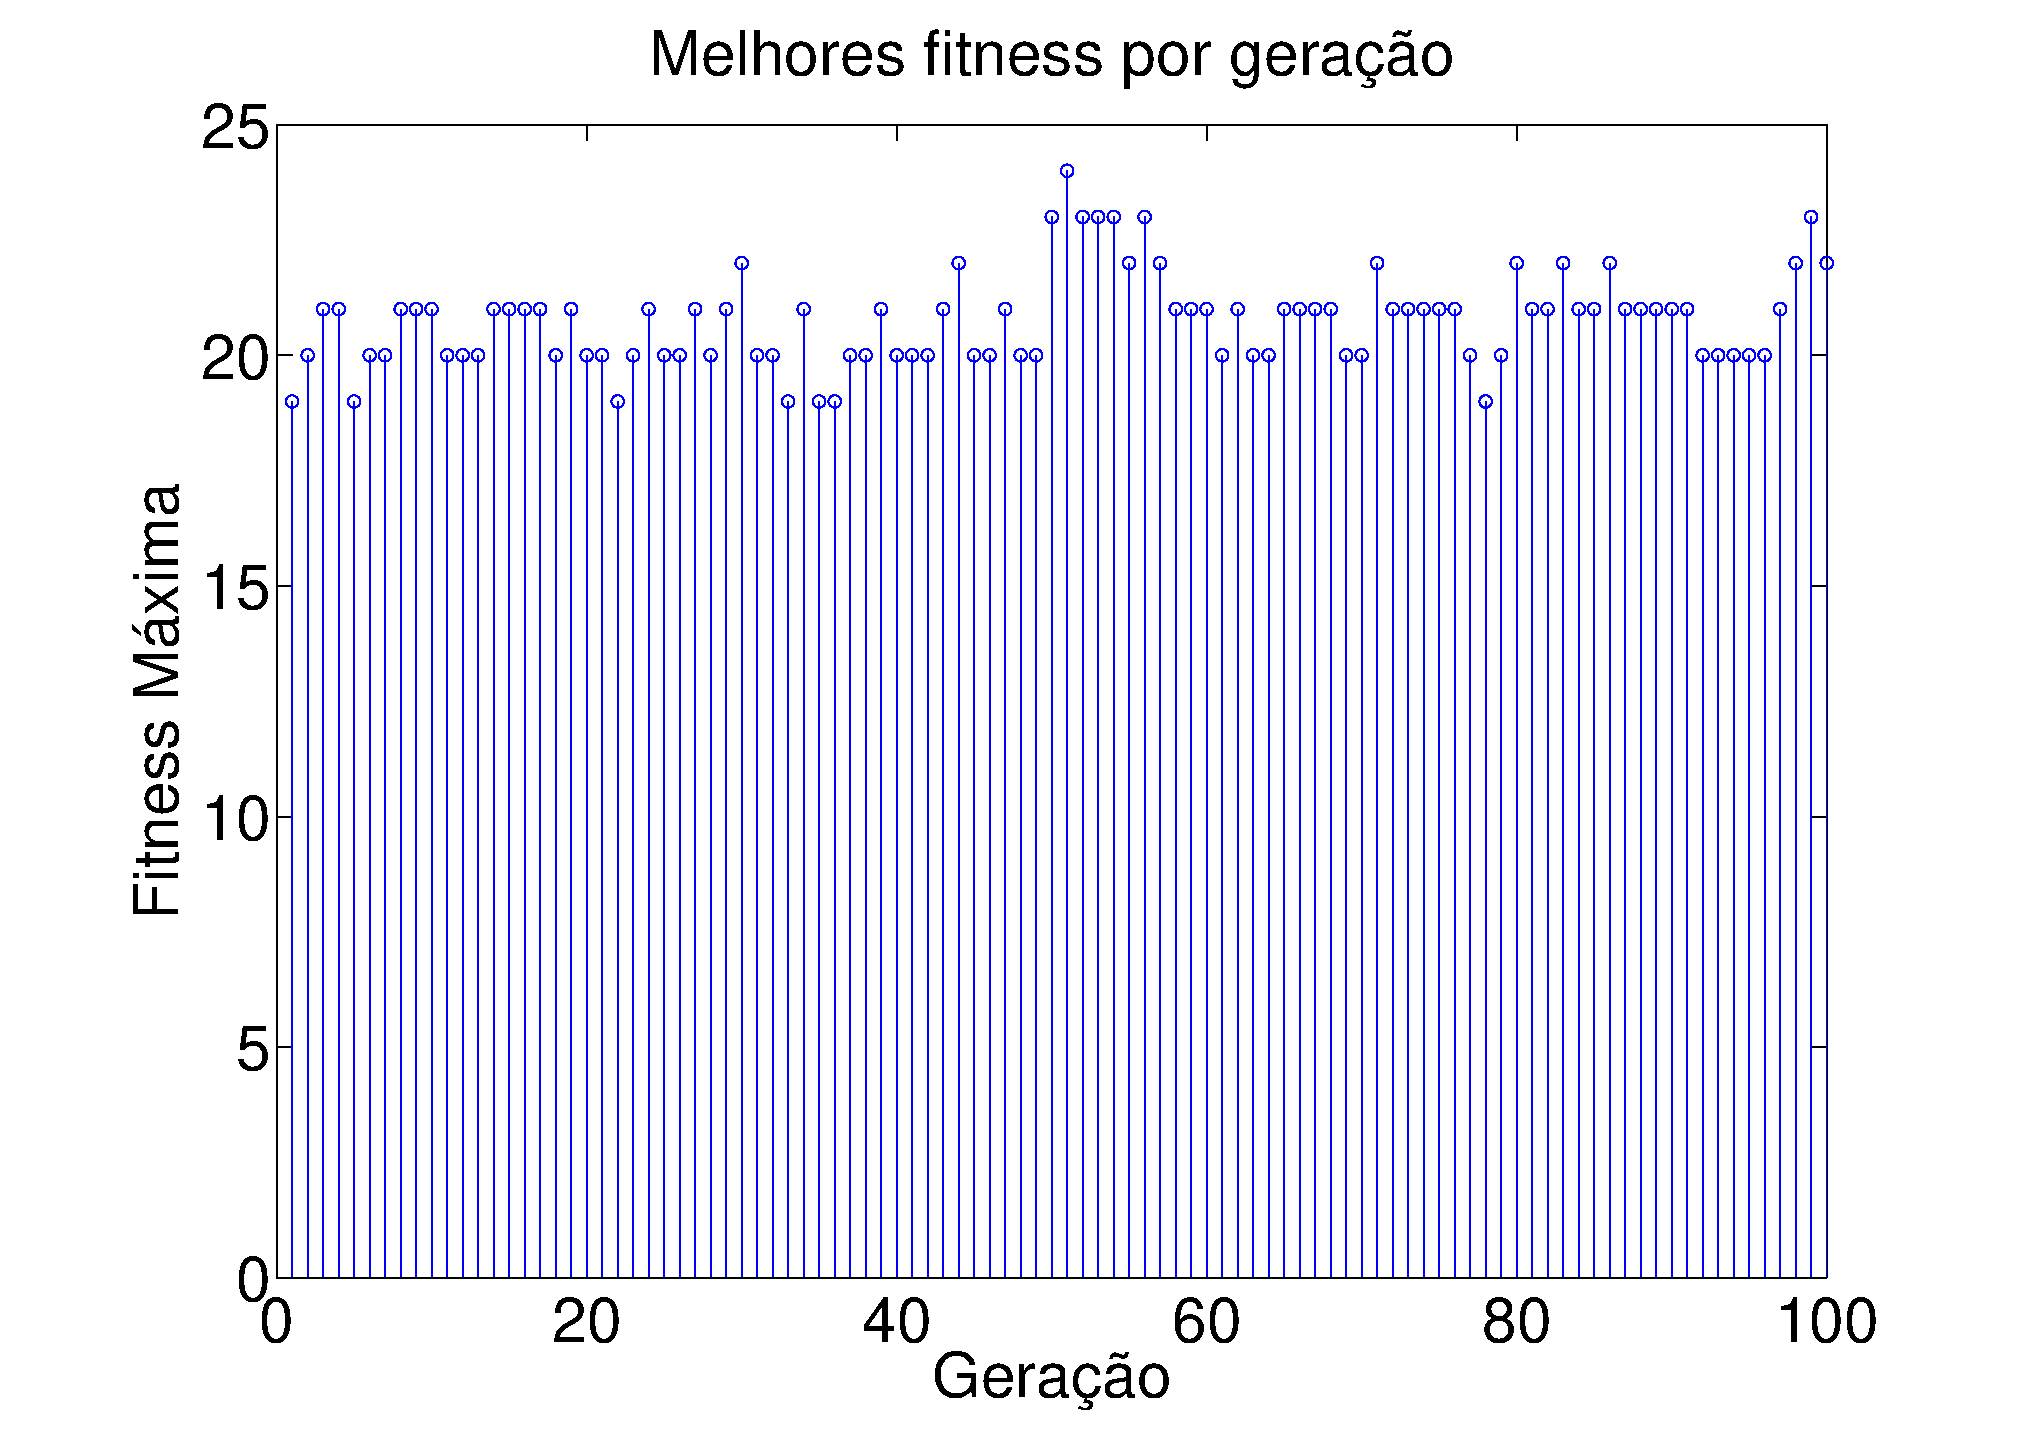
\includegraphics[width = 0.8\textwidth]{Q02_maximos_fitness_100_ger_nao_memetico.eps}
	\caption{Valores máximos de fitness encontrados em cada geração (não memético)}
	\label{Q02_maximos_fitness_100_ger_nao_memetico}
\end{figure}   

\begin{figure}[H]
	\centering
	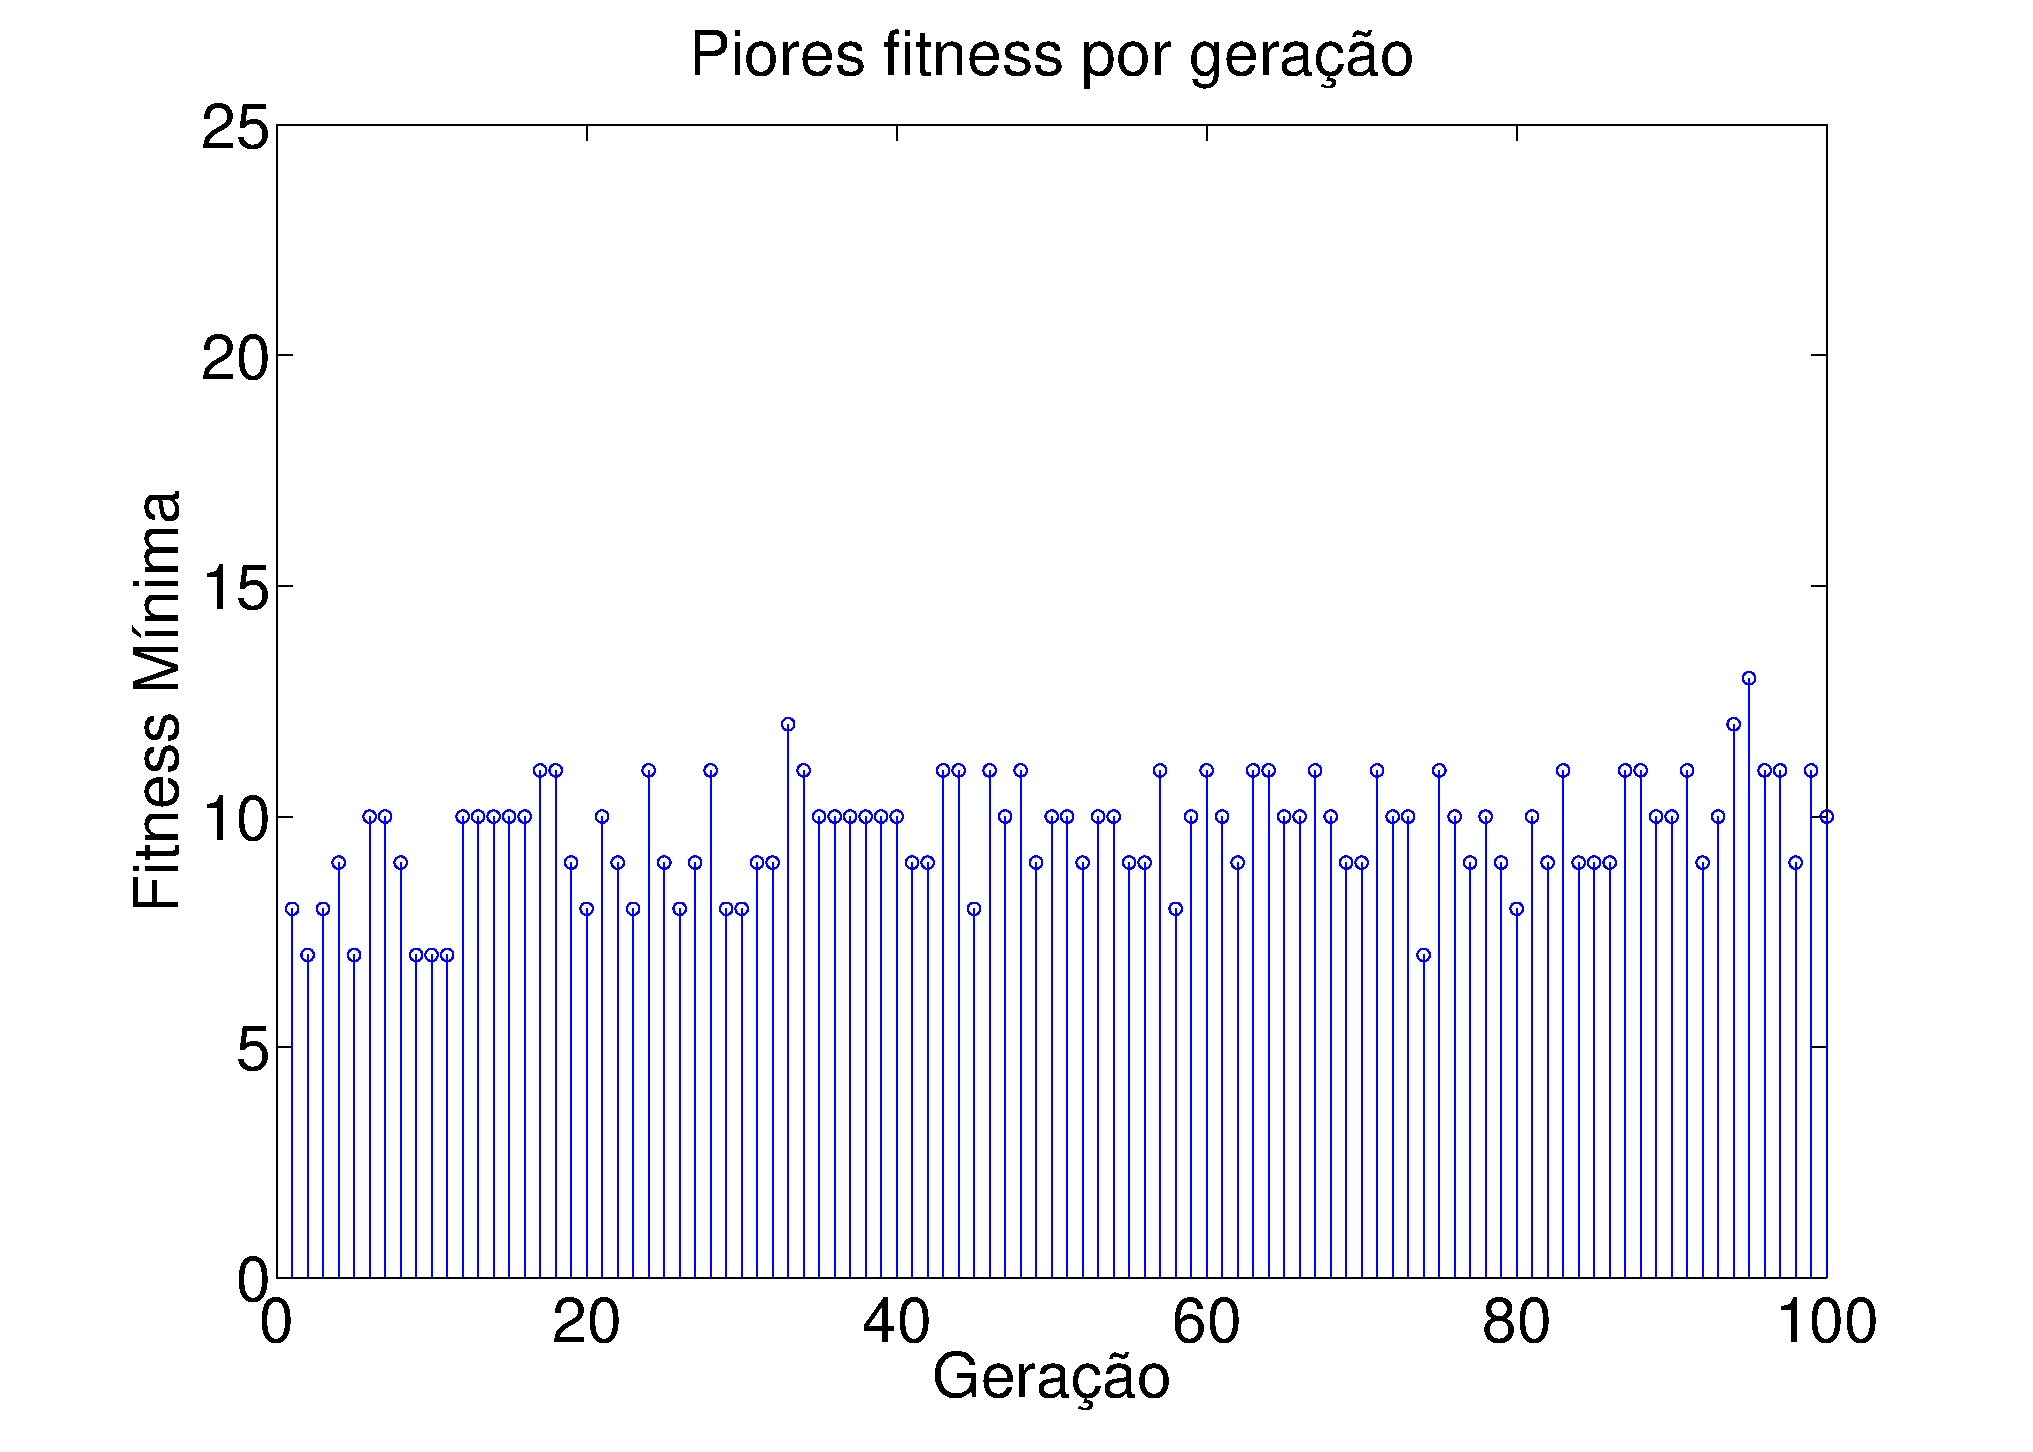
\includegraphics[width = 0.8\textwidth]{Q02_minimos_fitness_100_ger_nao_memetico.eps}
	\caption{Valores mínimos de fitness encontrados em cada geração (não memético)}
	\label{Q02_minimos_fitness_100_ger_nao_memetico}
\end{figure}   

\begin{figure}[H]
	\centering
	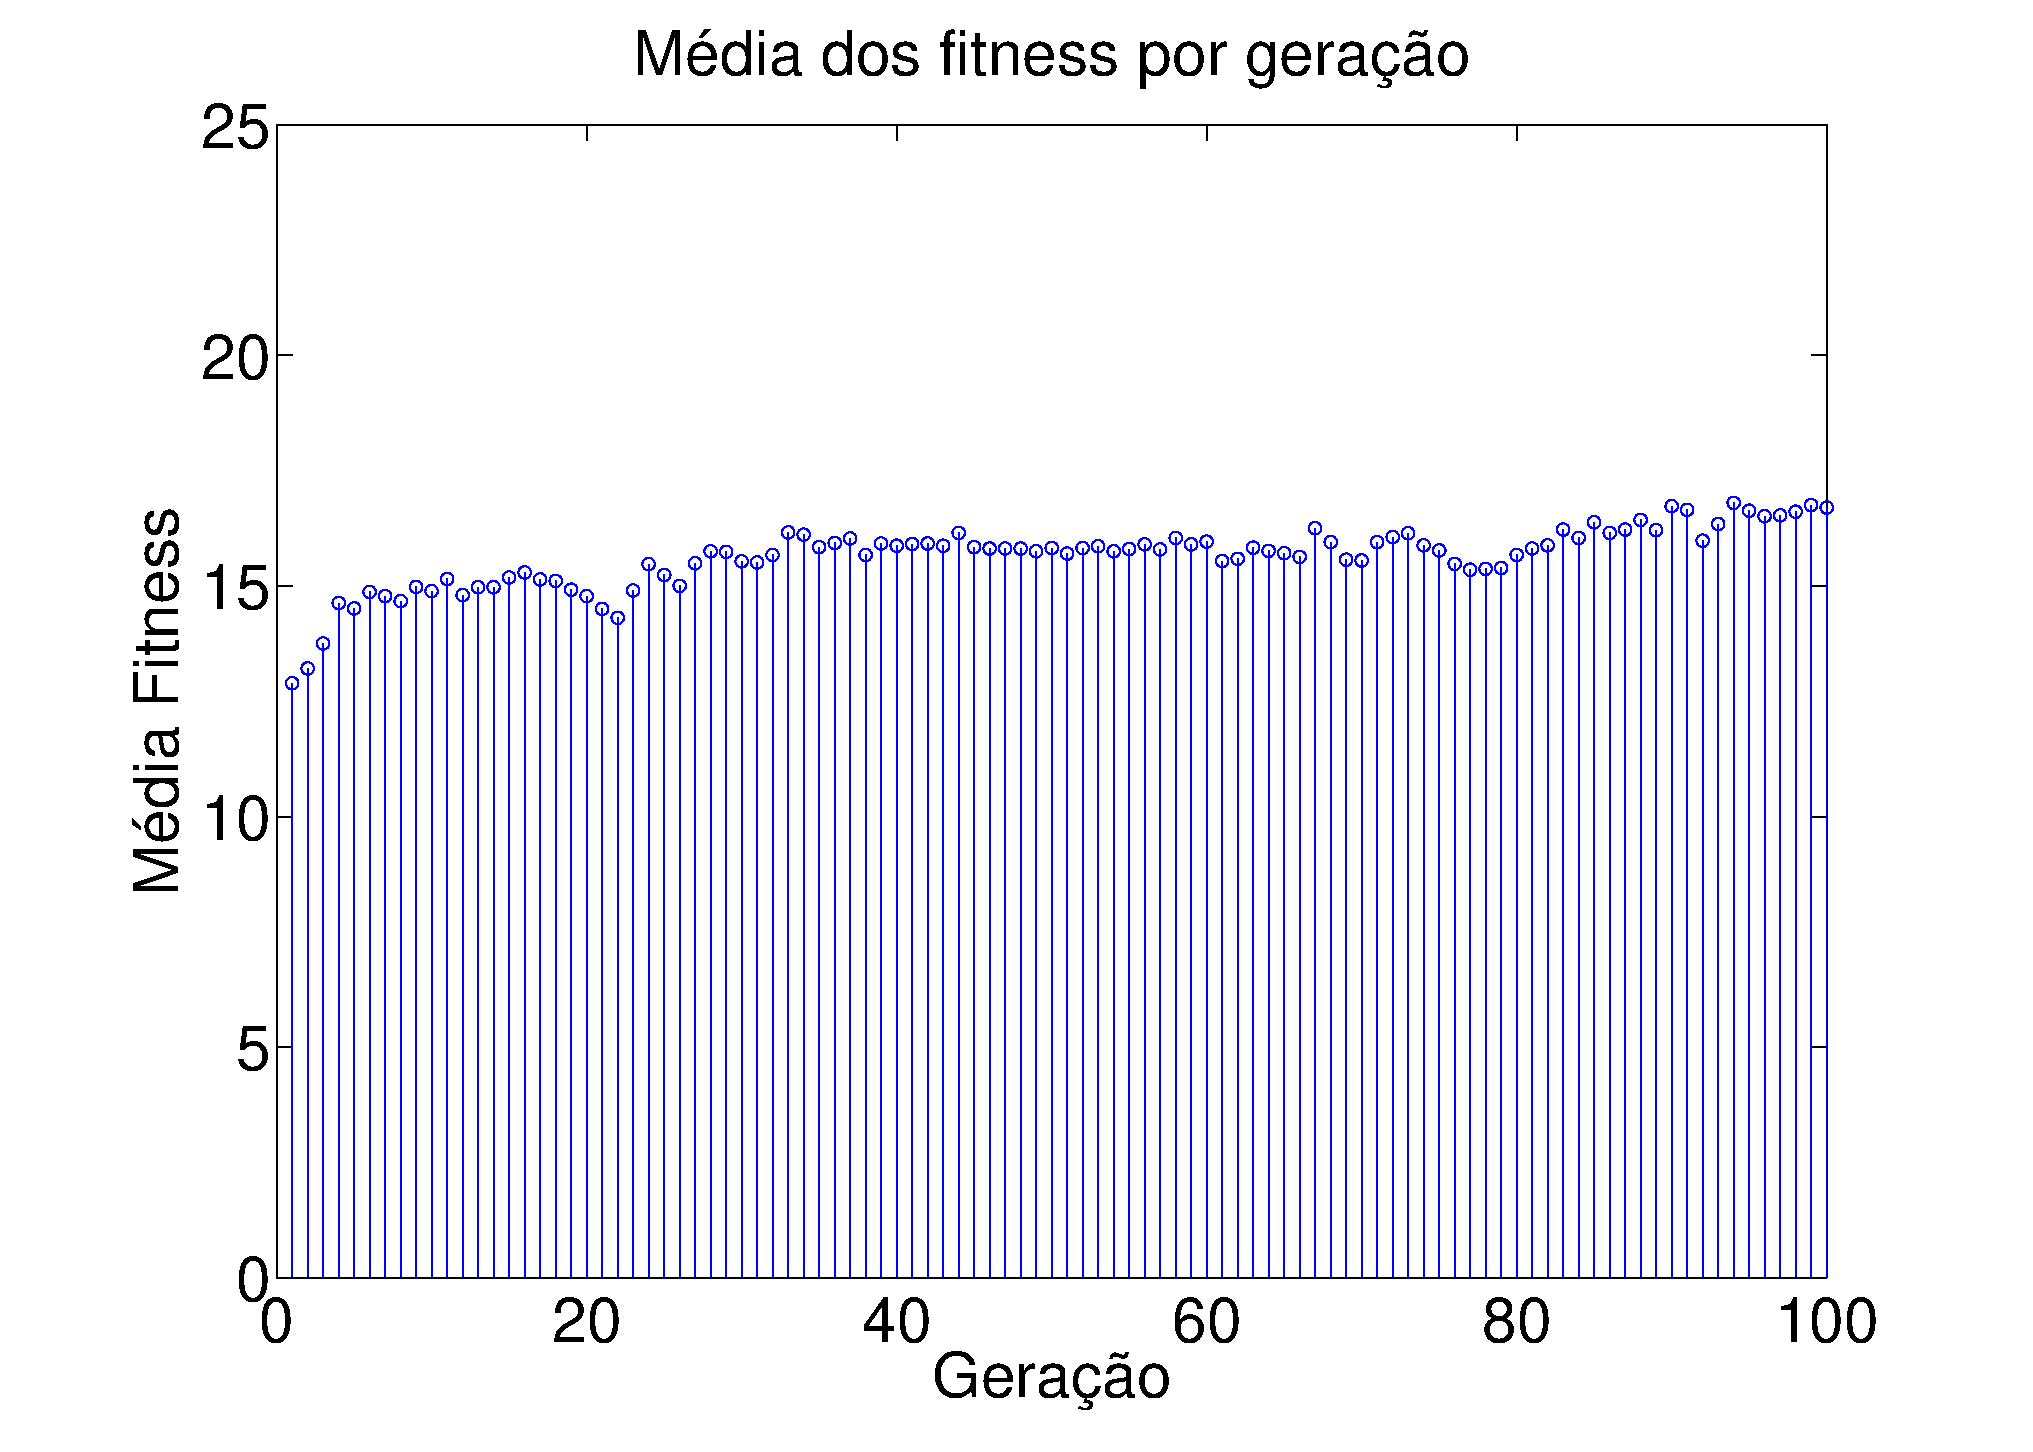
\includegraphics[width = 0.8\textwidth]{Q02_medias_fitness_100_ger_nao_memetico.eps}
	\caption{Valores médios de fitness encontrados em cada geração (não memético)}	
	\label{Q02_medias_fitness_100_ger_nao_memetico}
\end{figure}   

\paragraph{} Mesmo realizando somente uma iteração na busca local, a introdução desse passo no algoritmo rendeu um desempenho melhor do que a versão anterior. De fato, das 10 execuções desse novo algoritmo, cada uma indo até, no máximo, 100 gerações, o máximo global foi alcançado em 1, ao contrário da versão anterior, em que em nenhuma das execuções esse valor foi encontrado. A Figura \ref{Q02_maximos_fitness_100_ger_baldwin} exibe uma execução, na qual o valor máximo foi encontrado em 29 gerações. As Figuras \ref{Q02_minimos_fitness_100_ger_baldwin} e \ref{Q02_medias_fitness_100_ger_baldwin} exibem, respectivamente, as fitness mínimas e médias encontradas ao longo das 29 gerações. É interessante notar que a média de fitness, ao longo das gerações, assim como no caso anterior, foi aumentando, sugerindo uma aproximação do algoritmo da solução ótima global. A média de gerações requeridas para se alcançar o máximo global, levando-se em conta as 10 execuções independentes do algoritmo, foi de 92.2, com desvio-padrão de 21.2 gerações. Essas figuras retratam a aplicação da abordagem de Baldwin para a busca local.\\

\begin{figure}[H]
	\centering
	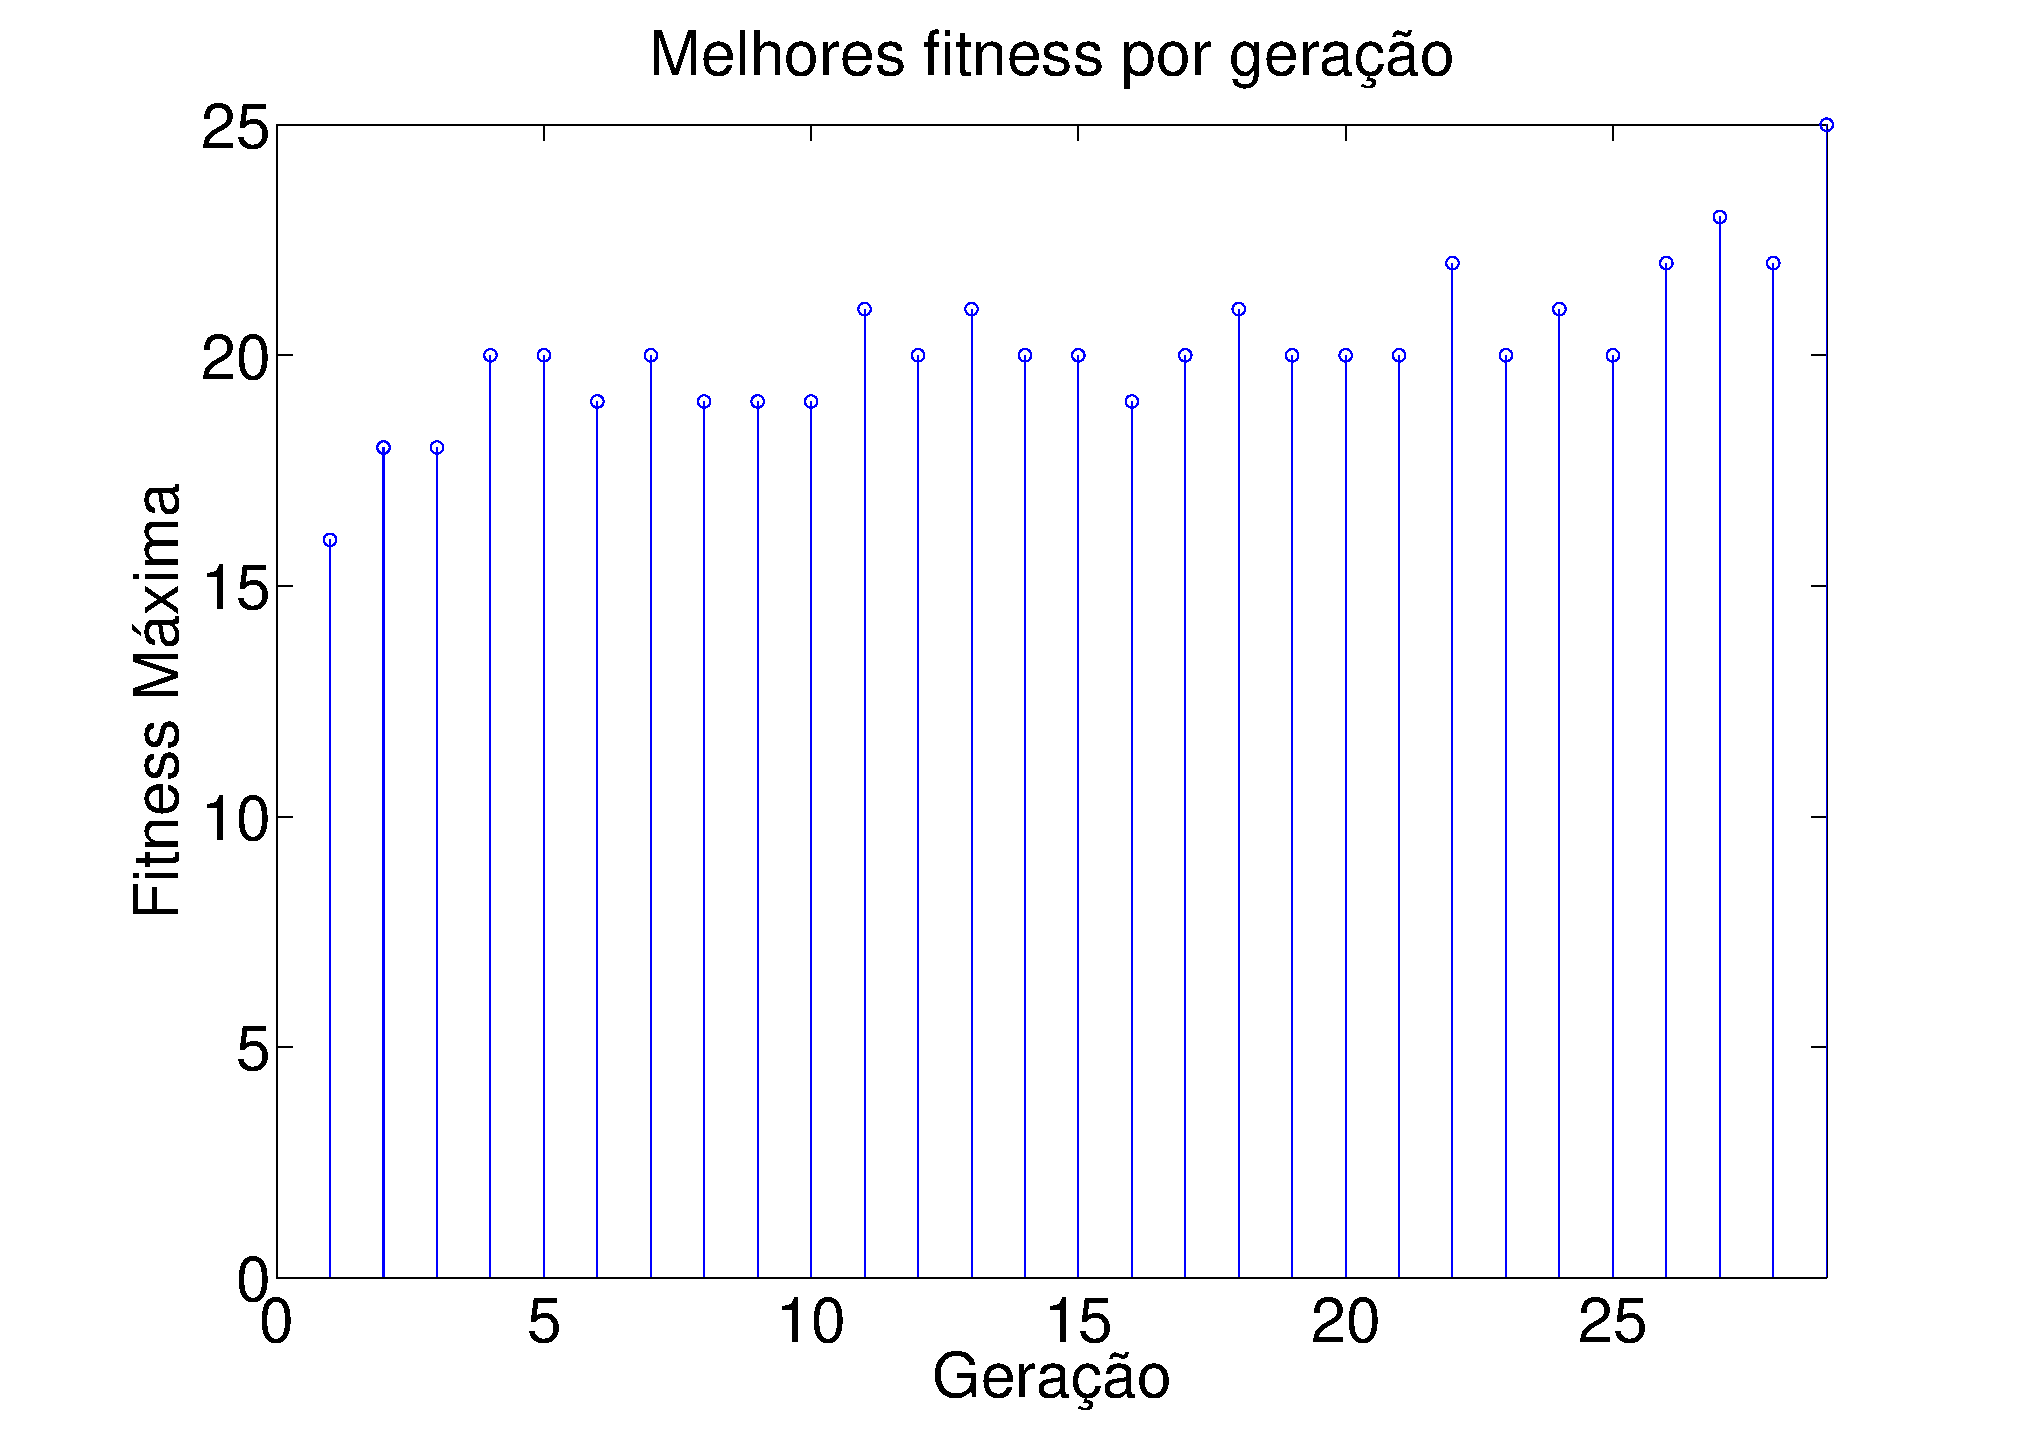
\includegraphics[width = 0.8\textwidth]{Q02_maximos_fitness_100_ger_baldwin.eps}
	\caption{Valores máximos de fitness encontrados em cada geração (Baldwin)}
	\label{Q02_maximos_fitness_100_ger_baldwin}
\end{figure}   

\begin{figure}[H]
	\centering
	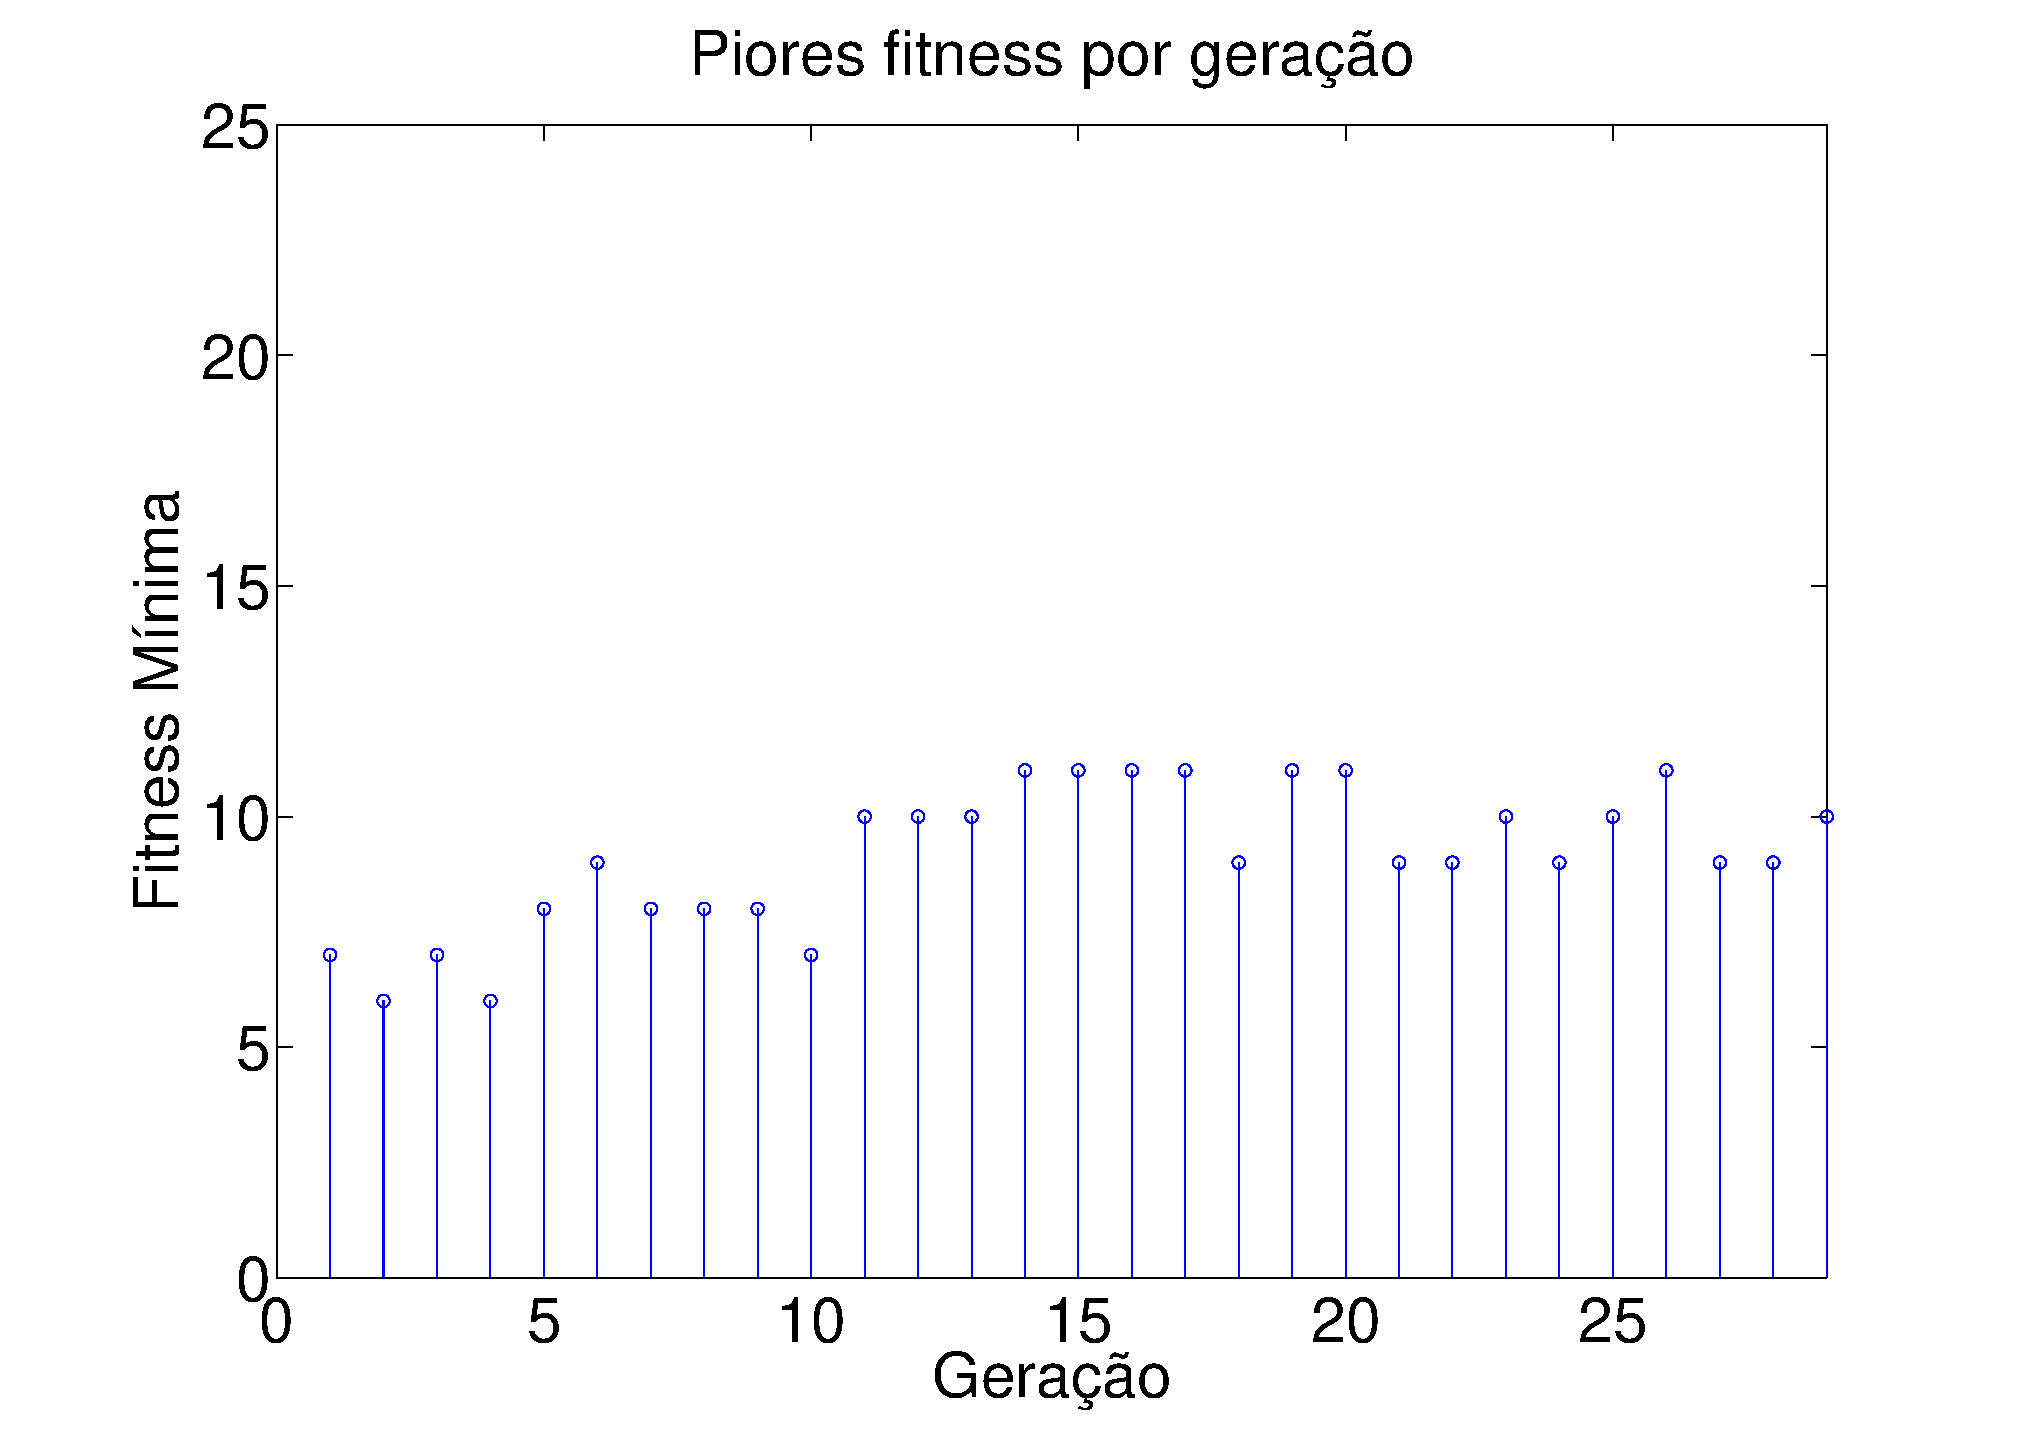
\includegraphics[width = 0.8\textwidth]{Q02_minimos_fitness_100_ger_baldwin.eps}
	\caption{Valores mínimos de fitness encontrados em cada geração (Baldwin)}
	\label{Q02_minimos_fitness_100_ger_baldwin}
\end{figure}   

\begin{figure}[H]
	\centering
	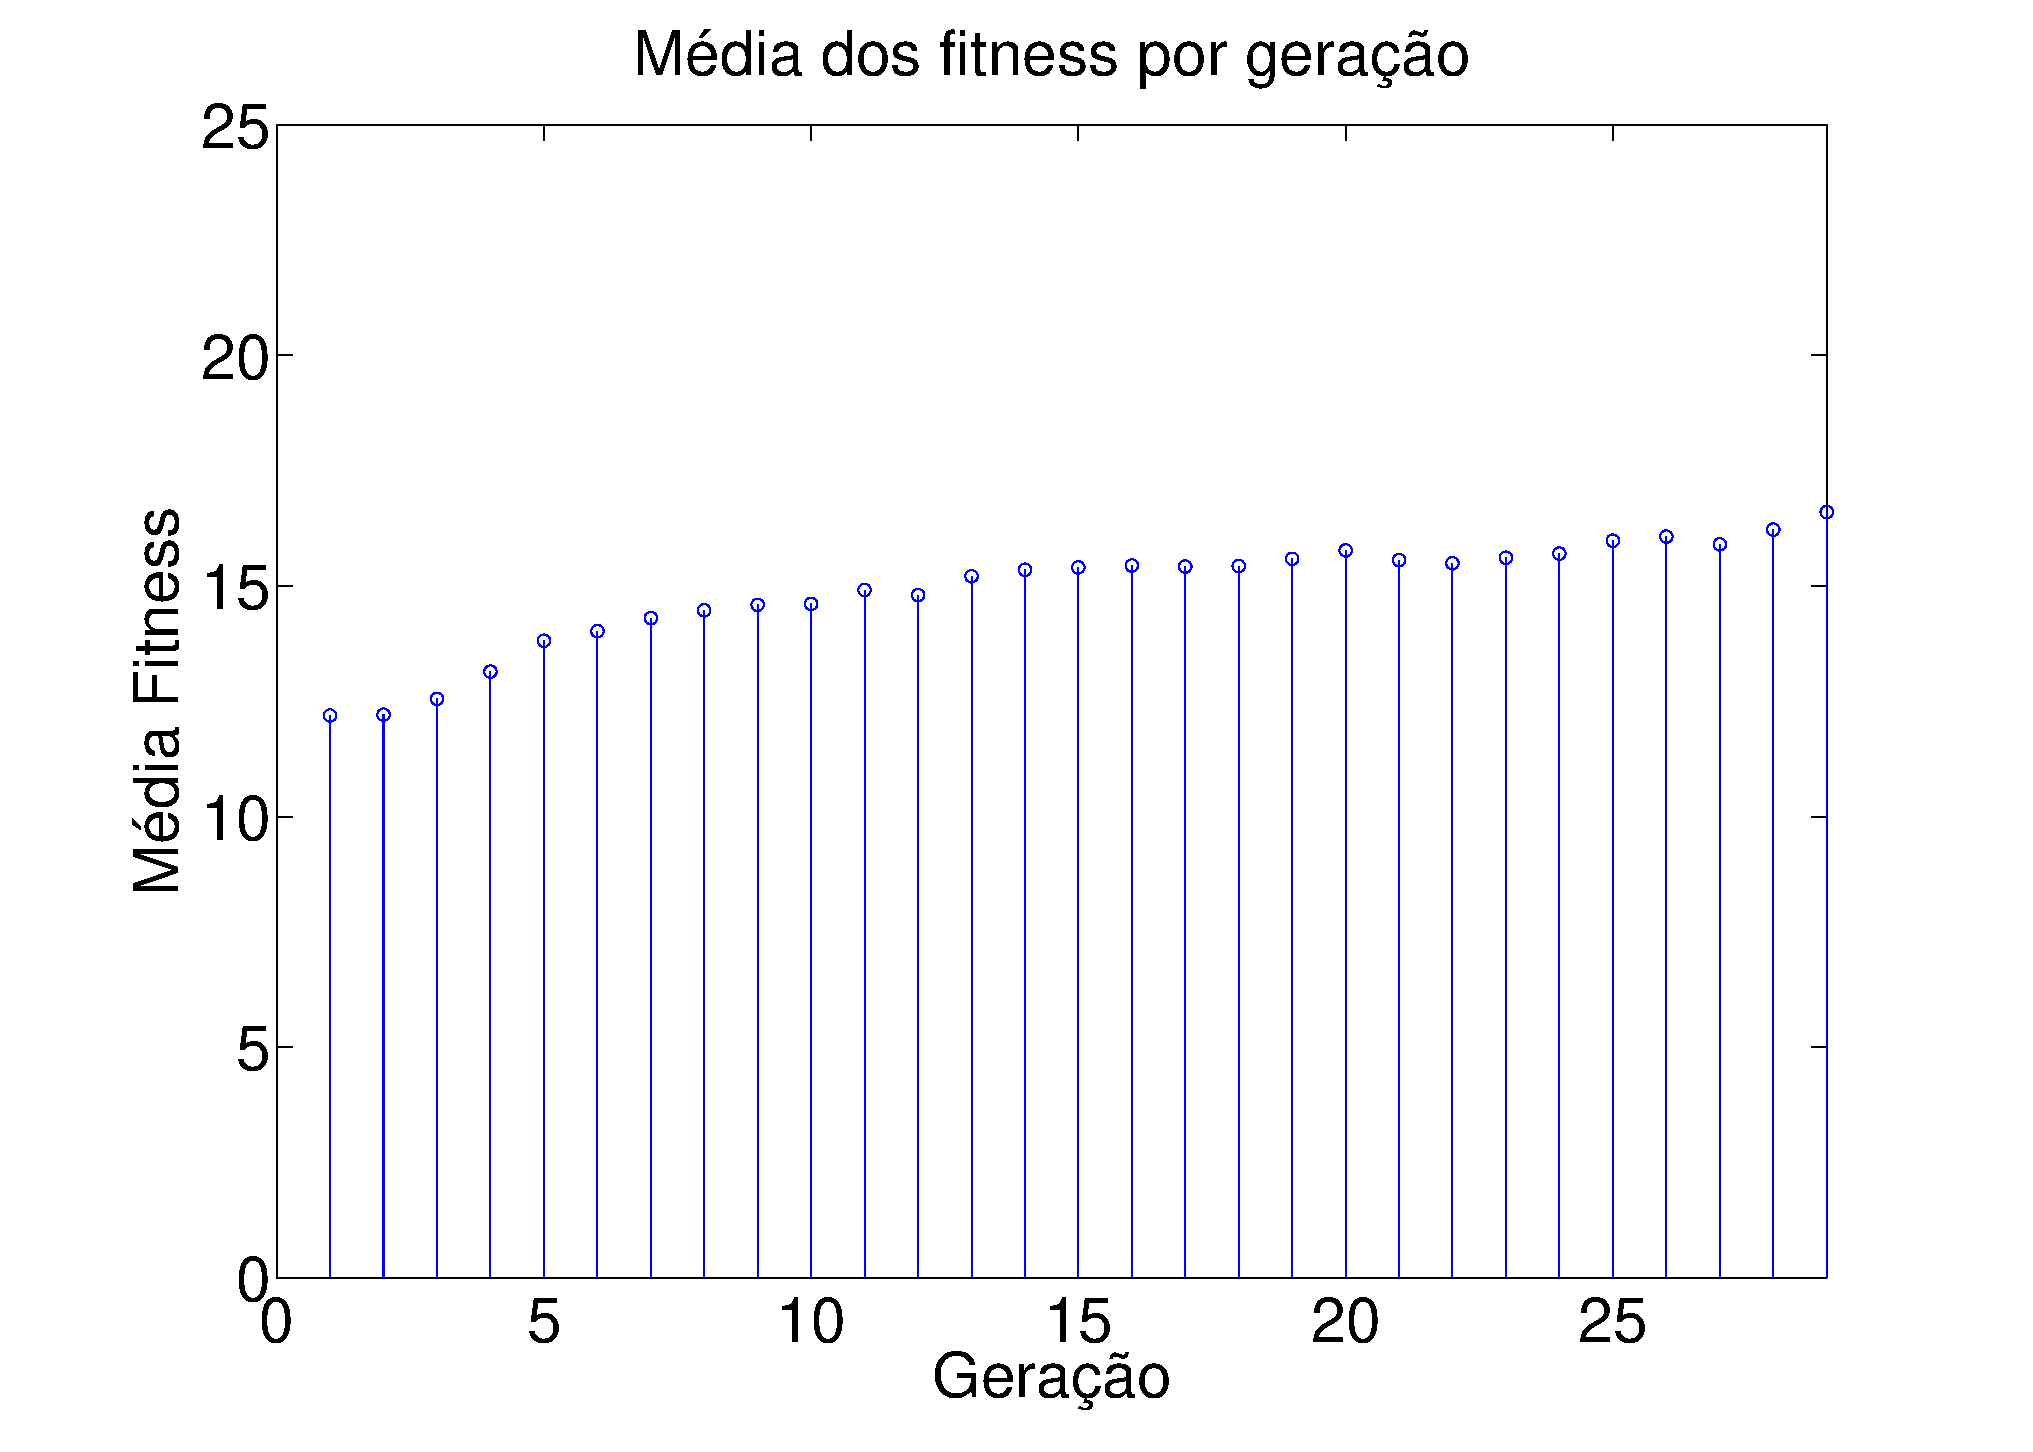
\includegraphics[width = 0.8\textwidth]{Q02_medias_fitness_100_ger_baldwin.eps}
	\caption{Valores médios de fitness encontrados em cada geração (Baldwin)}	
	\label{Q02_medias_fitness_100_ger_baldwin}
\end{figure}   

\paragraph{} Já as Figuras \ref{Q02_maximos_fitness_100_ger_lamarck}, \ref{Q02_minimos_fitness_100_ger_lamarck} e \ref{Q02_medias_fitness_100_ger_lamarck} exibem os valores máximos, mínimos e médios das fitness encontradas ao longo de cada geração, durante uma execução do algoritmo, utilizando-se a abordagem de Lamarck. Vale ressaltar que os resultados encontrados utilizando essa abordagem foram melhores do que aqueles obtidos pela abordagem de Baldwin. Nesse caso, o ótimo global foi encontrado em 2 das 10 execuções, requerendo, em média, 90.9 gerações para se alcançar essa solução, com um desvio-padrão de 24.1 gerações.\\

\begin{figure}[H]
	\centering
	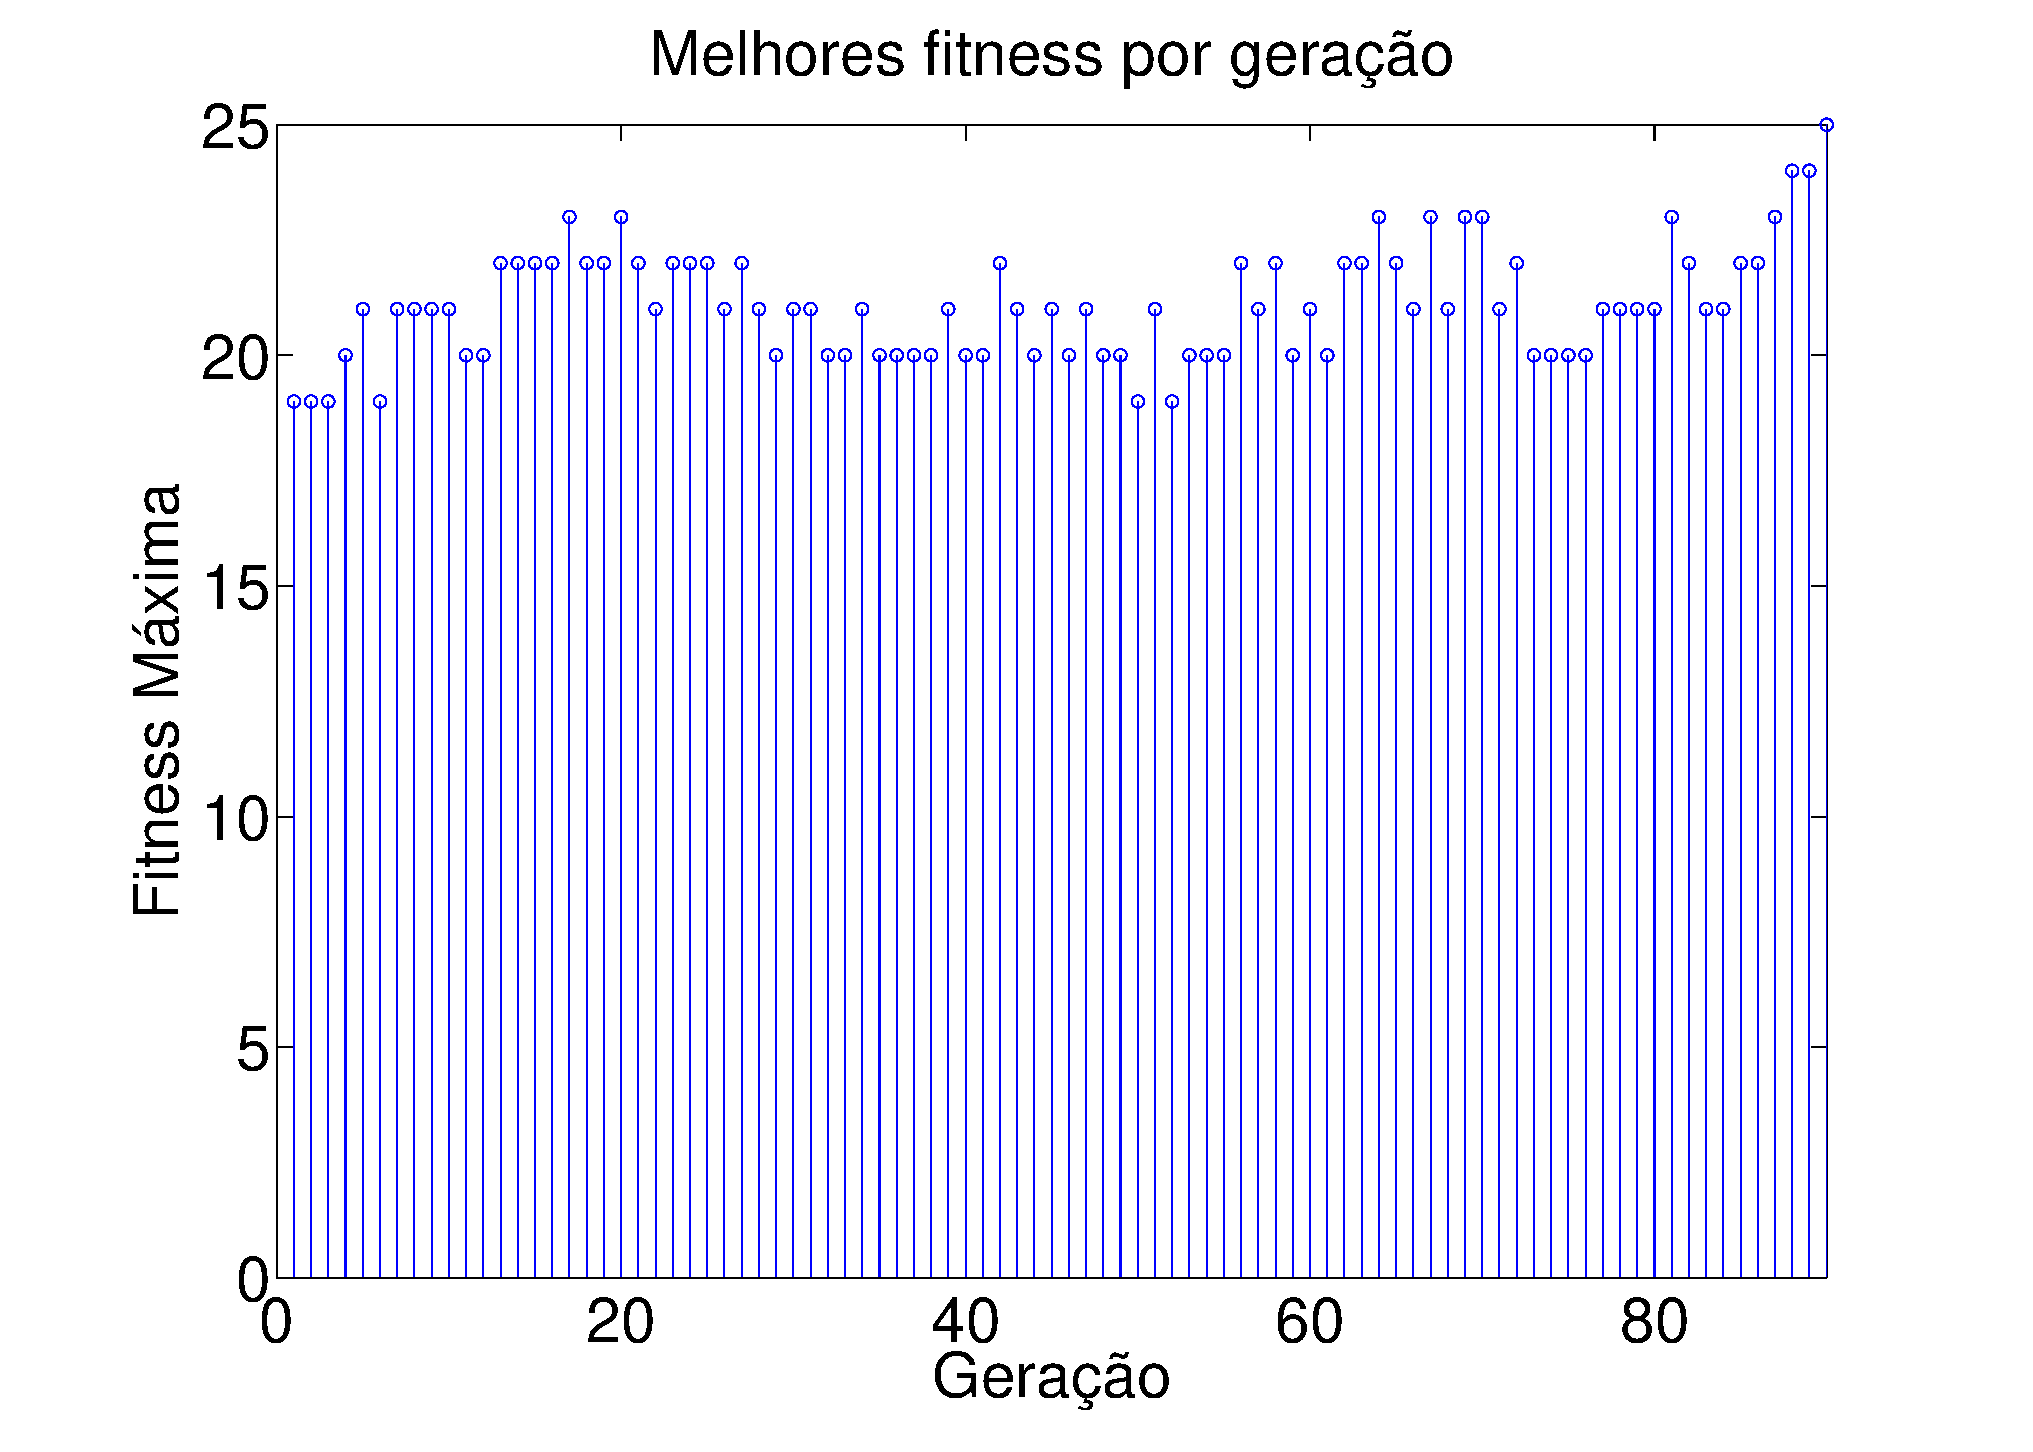
\includegraphics[width = 0.8\textwidth]{Q02_maximos_fitness_100_ger_lamarck.eps}
	\caption{Valores máximos de fitness encontrados em cada geração (Lamarck)}
	\label{Q02_maximos_fitness_100_ger_lamarck}
\end{figure}   

\begin{figure}[H]
	\centering
	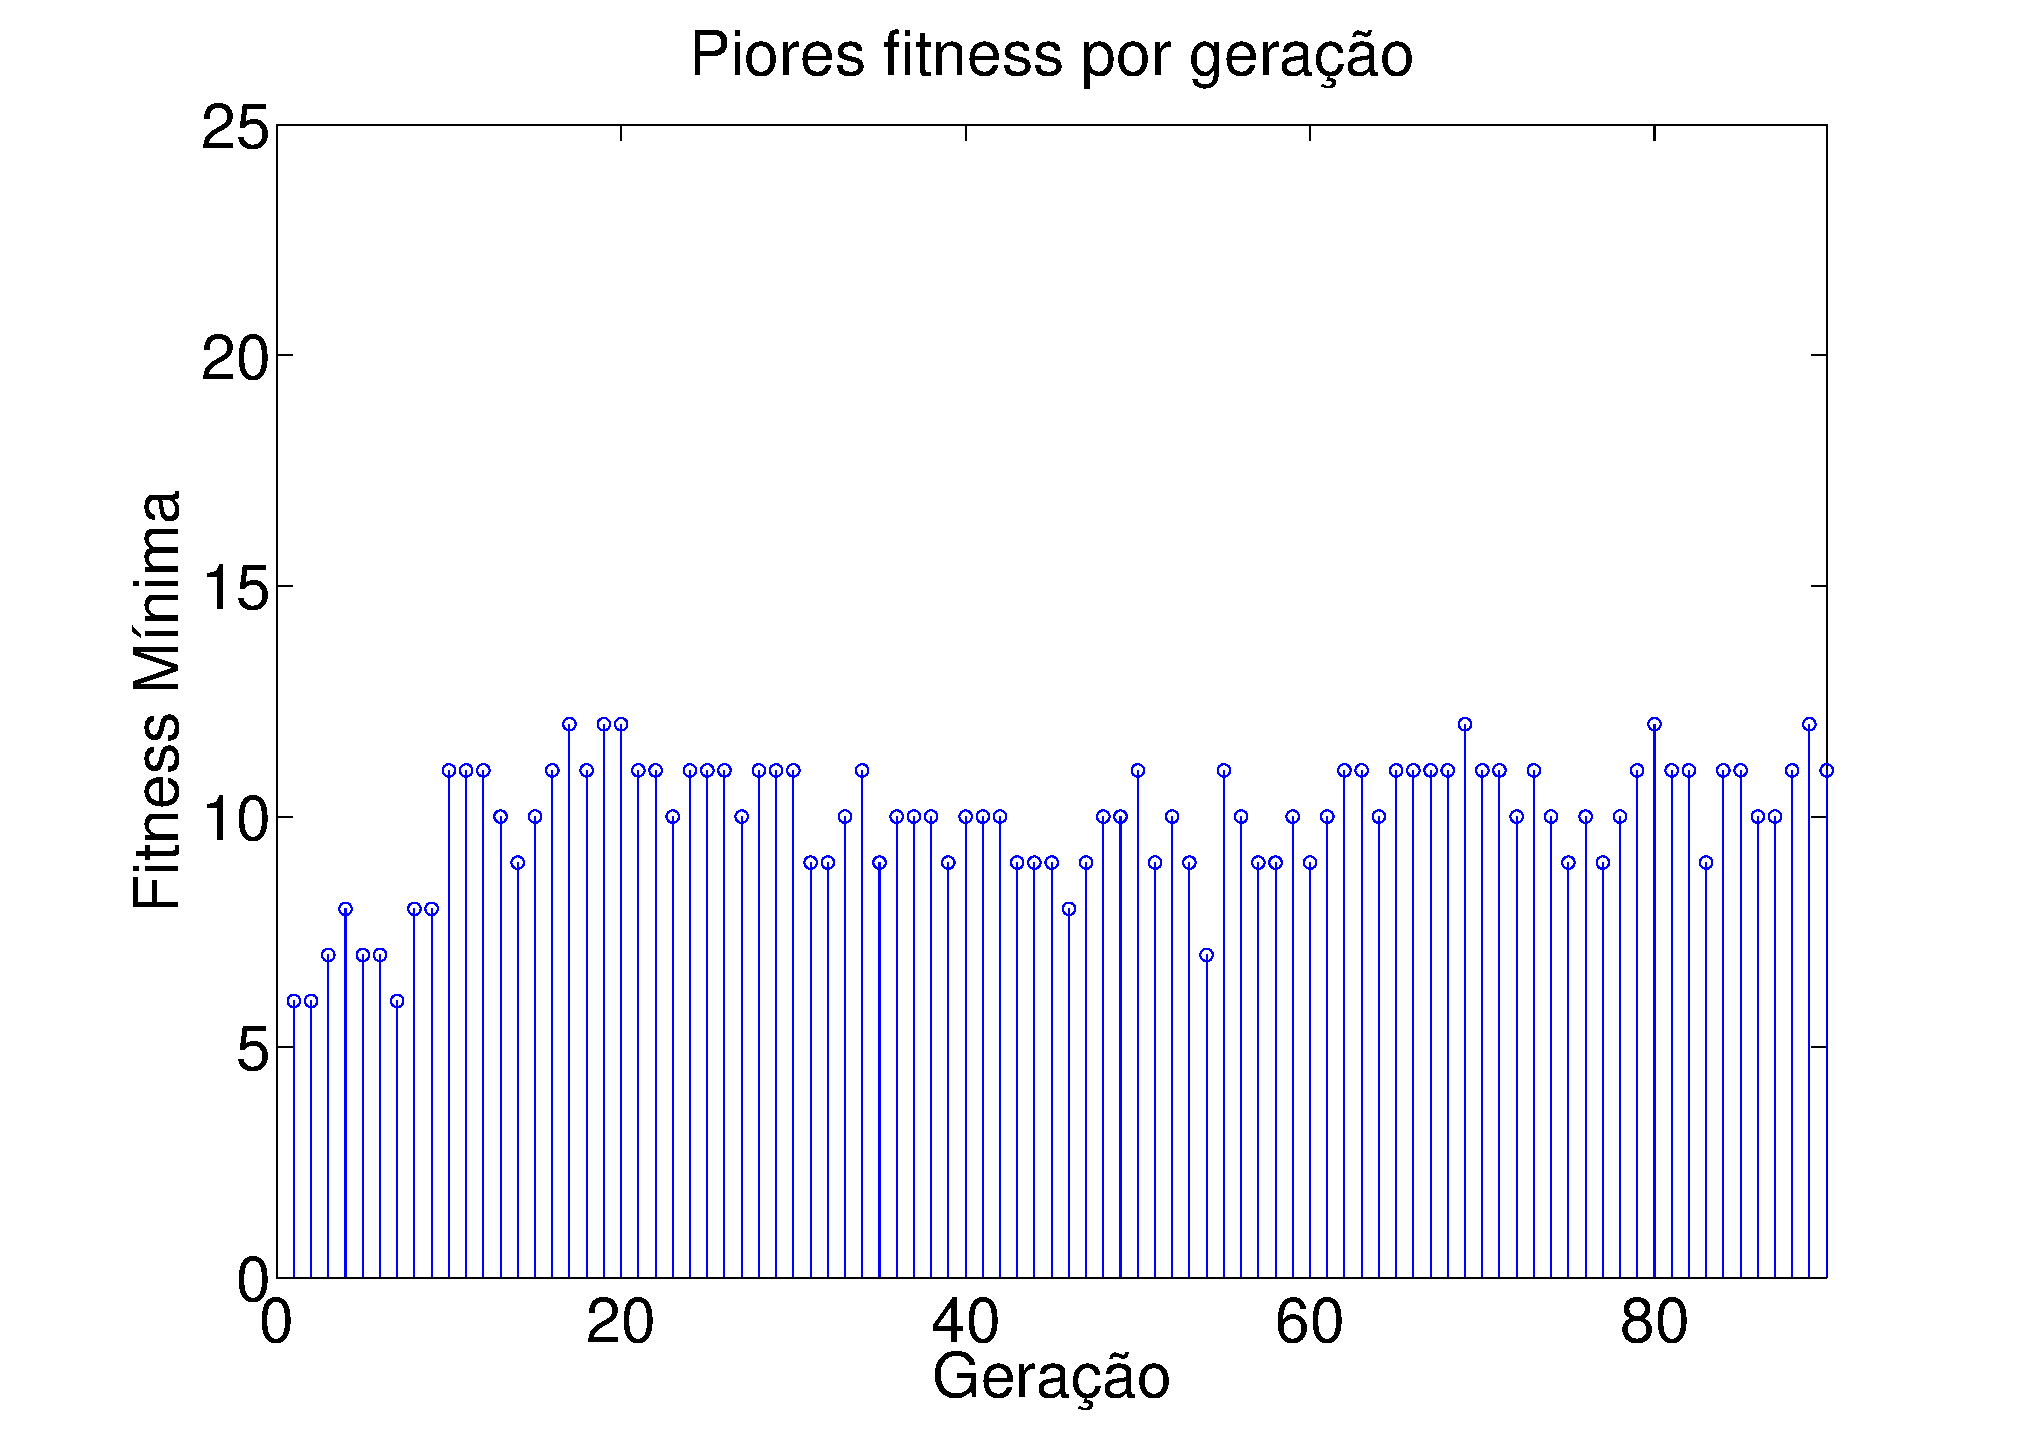
\includegraphics[width = 0.8\textwidth]{Q02_minimos_fitness_100_ger_lamarck.eps}
	\caption{Valores mínimos de fitness encontrados em cada geração (Lamarck)}
	\label{Q02_minimos_fitness_100_ger_lamarck}
\end{figure}   

\begin{figure}[H]
	\centering
	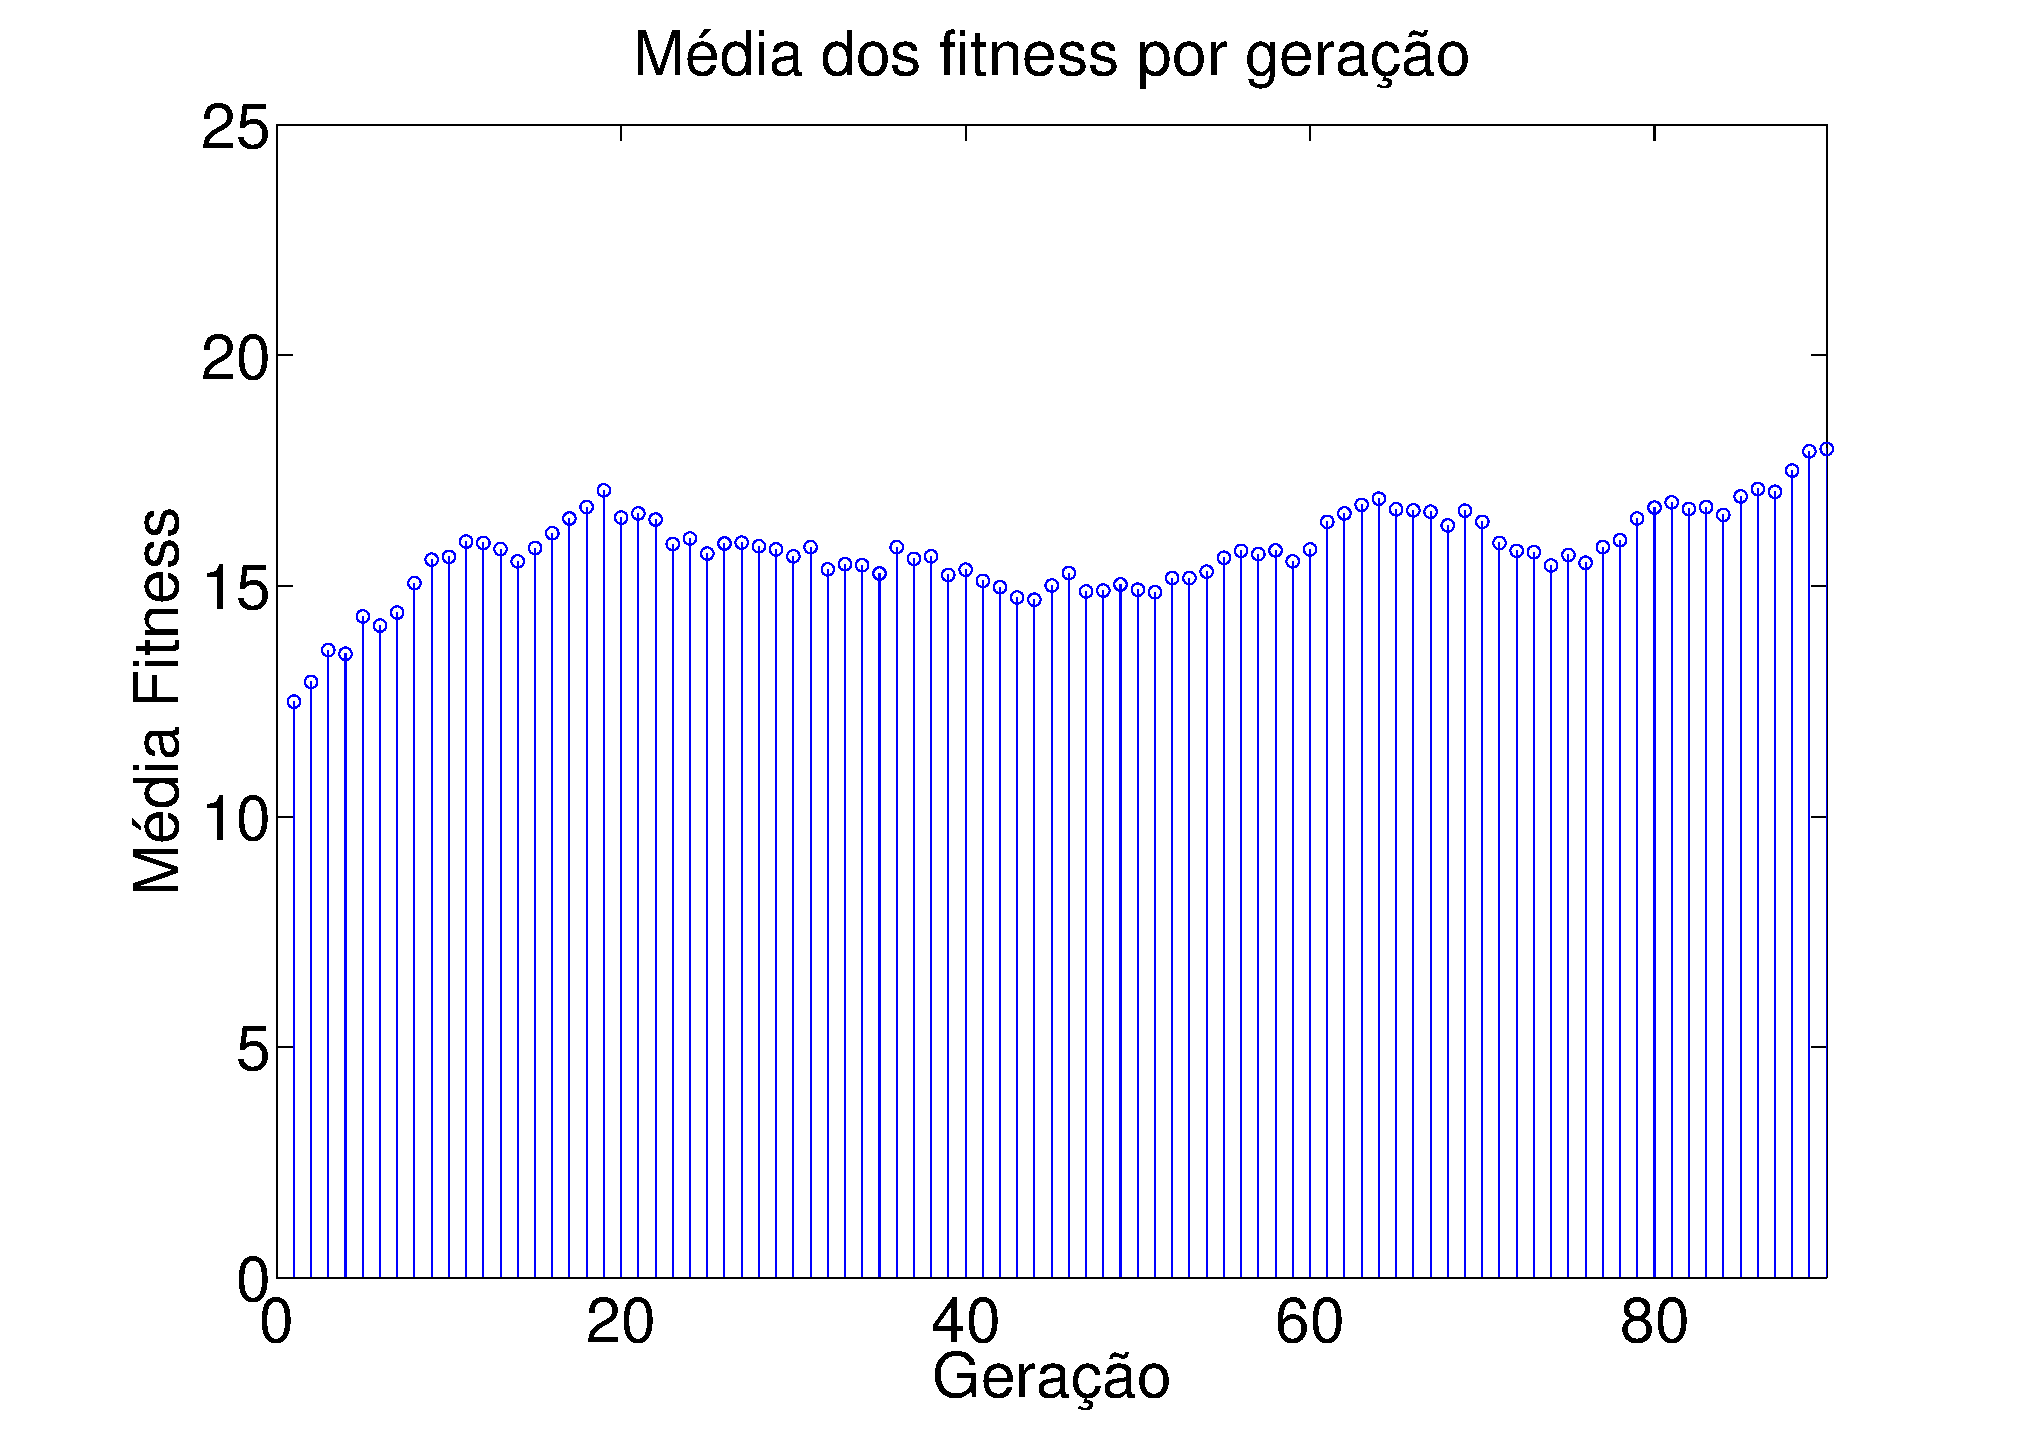
\includegraphics[width = 0.8\textwidth]{Q02_medias_fitness_100_ger_lamarck.eps}
	\caption{Valores médios de fitness encontrados em cada geração (Lamarck)}	
	\label{Q02_medias_fitness_100_ger_lamarck}
\end{figure}   

\section*{Questão 3}

\textbf{\textit{Capítulo 12, Exercício 1:}}\\

\textbf{Specify the eight-queens problem as a CSP $\left<S,\phi\right>$.}\\

\paragraph{} O problema das oito rainhas é naturalmente pensado como um problema de satisfação de restrições, já que somente são consideradas soluções válidas aquelas, nas quais nenhuma das oito rainhas é atacada por outra (ou seja, não outras rainhas presentes nas direções vertical, horizontal e diagonal da rainha em questão). De modo a formalizar a definição desse problema como um CSP (\textit{``Constrained Satisfaction Problem"}), define-se dois parâmetros: o espaço de busca $S$ e a restrição $\phi$ a ser respeitada.\\

\begin{itemize}

	\item[\textbf{1.}] Definição do espaço de busca $S$
	
	\paragraph{} O espaço de busca $S$, ao qual pertencem as possíveis soluções do problema, pode ser definido de diversas formas. Uma maneira, por exemplo, seria $S = (l,c)^{8}$, onde $l, c \in \{1, 2, 3, 4, 5, 6, 7, 8\}$. Nesse caso, como o tabuleiro de xadrez tem tamanho $8 \times 8$, são precisos 8 pares-ordenados $(l,c)$ para definir uma solução, já que cada um deles define a posição de uma rainha (linha e coluna, respectivamente). Vale ressaltar que esse espaço de soluções apresenta uma quantidade elevada de soluções inválidas, uma vez que nenhuma restrição é implicitamente imposta sobre ele. Caso se adote esse espaço, o controle sobre as restrições do problema deverá ser feito de forma explícita, ou seja, não aceitar soluções desse espaço que infrinjam alguma restrição. Para exemplificar, a solução $\{(1,2),(1,3),(2,2),(5,5),(8,4),(7,1),(4,6),(3,8)\}$ não seria válida, já que mais de uma rainha em uma linha ou coluna não é permitido.
	
	\paragraph{} Alternativamente, é possível adicionar implicitamente uma restrição no espaço de soluções, de modo que o novo espaço gerado apresenta, somente, soluções que automaticamente respeitam a restrição imposta. Sendo assim, o espaço de busca poderia ser definido como $S = C^{8}$, onde $C = \{1, 2, 3, 4, 5, 6, 7, 8 \}$. Nesse caso, $C$ define a coluna sobre a qual uma rainha será colocada (como são 8 colunas, o espaço de busca fica $C^{8}$), ao passo que os números que definem esse conjunto correspondem ao índice da linha sobre a qual a rainha da coluna se situa. Note que, com essa nova definição de espaço, a restrição de que nenhuma coluna pode conter mais de uma rainha é automaticamente satisfeita. 
	
	\paragraph{} A definição anterior contempla a restrição das colunas, porém, deixa em aberto a restrição das linhas e das diagonais, sendo necessário, portanto, a validação explicíta dessas condições, antes do algoritmo aceitar tais soluções. No entanto, é possível, ainda, definir o espaço de uma outra forma, de modo a incluir a restrição das linhas (nenhuma linha pode conter mais do que uma rainha), através da seguinte forma: $S = \{s_1, s_2, \ ..., s_8\}$, onde $s_i \in \{1, 2, 3, 4, 5, 6, 7, 8 \}$ e $\forall i, j \in \{1, 2, 3, 4, 5, 6, 7, 8\}, s_i \neq s_j$. O índice $i$ representa o número da coluna, enquanto que $s_i$ representa o número da linha em que se localiza a rainha da coluna $i$. Em outras palavras, o espaço anterior é definido como uma permutação de números não-repetidos entre 1 e 8. Nesse caso, a restrição das linhas é automaticamente satisfeita, pois, como os números não são repetidos, não há como soluções desse espaço representarem rainhas em linhas iguais. Adotando esse espaço reduzido como o de busca, resta somente ao algoritmo checar explicitamente a condição das diagonais, antes de validar uma solução. A vantagem de definir restrições implicitamente é que isso poupa tempo de processamento do algoritmo, uma vez que ele gasta menos tempo na região de soluções inválidas do problema.\\
	
	\item[\textbf{2.}] Definição da restrição $\phi$
	
	\paragraph{} A restrição $\phi$ para o problema das oito rainhas pode ser definida como uma composição de 3 restrições, conforme já apontado anteriormente: de linhas, de colunas e de diagonais.
	
	\begin{itemize}
		
		\item[1.] $r_l = verdadeiro$, se não houver mais do que uma rainha presente em uma linha;
		
		\item[2.] $r_c = verdadeiro$, se não houver mais do que uma rainha presente em uma coluna;
		
		\item[3.] $r_d = verdadeiro$, se não houver mais do que uma rainha presente em uma diagonal.	
		
	\end{itemize}
	
	\paragraph{} Dessa forma, a restrição $\phi$ será verdadeira, se, e somente se, as 3 outras restrições forem verdadeiras: $\phi(\overline{s}) = verdadeiro \iff r_l \wedge r_c \wedge r_d = verdadeiro$ ($\wedge$ é o operador lógico matemático \textit{``AND"} (``E")).\\
	 
\end{itemize}

\paragraph{} Com a caracterização dos parâmetros $S$ e $\phi$, conclui-se a especificação do problema das oito rainhas como um CSP.\\

\section*{Questão 4}

\textbf{Escreva (utilizando um pseudo-código) um algoritmo genético simples para a solução do Exercício 4 da Lista de Exercícios \#5, considerando que a população não é de dicionários $\mathbf{Y}$, mas sim de matrizes $p_{\mathbf{y}|\mathbf{x}}$ descrevendo as probabilidades com as quais um vetor de dados $\mathbf{x}$ é atribuído a um agrupamento $\mathbf{y}$.}\\

\paragraph{}

\end{document}